\documentclass{article}

\usepackage{tikz}
\title{Drawings with TikZ: Exercise}
\author{Donald Leung (Kellett)}
\date{\today}

\begin{document}

\maketitle

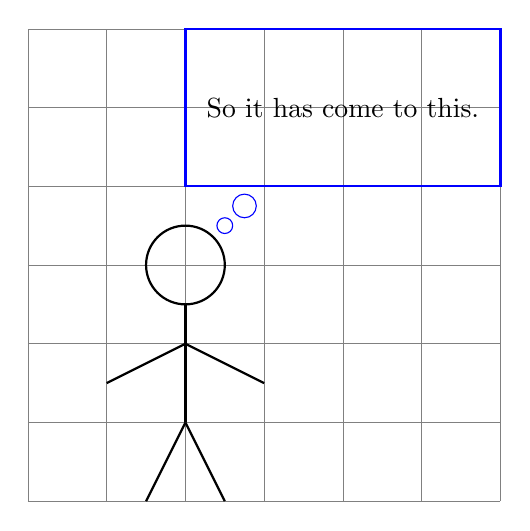
\begin{tikzpicture}

\draw[help lines] (0,0) grid (6,6);

\draw[thick] (1.5,0) -- (2,1);

\draw[thick] (2,1) -- (2.5,0);

\draw[thick] (2,1) -- (2,2.5);

\draw[thick] (2,3) circle (0.5);

\draw[thick] (2,2) -- (1,1.5);

\draw[thick] (2,2) -- (3,1.5);

\draw[blue] (2.5,3.5) circle (0.1);

\draw[blue] (2.75,3.75) circle (0.15);

\draw[blue, thick] (2,4) -- (2,6) -- (6,6) -- (6,4) -- cycle;

\node (t) at (4,5) {So it has come to this.};

\end{tikzpicture}

\end{document}